\section{Модели, положенные в основу разрабатываемого программного средства}
\label{sec:models:intro}


\subsection{Функциональная модель программного средства}
\label{sub:models:func_model}

Для представления функциональной модели была выбрана диаграмма вариантов использования UML, которая отражает отношения между актерами и прецедентами и позволяет описать систему на концептуальном уровне.

\begin{figure}[ht]
\centering
  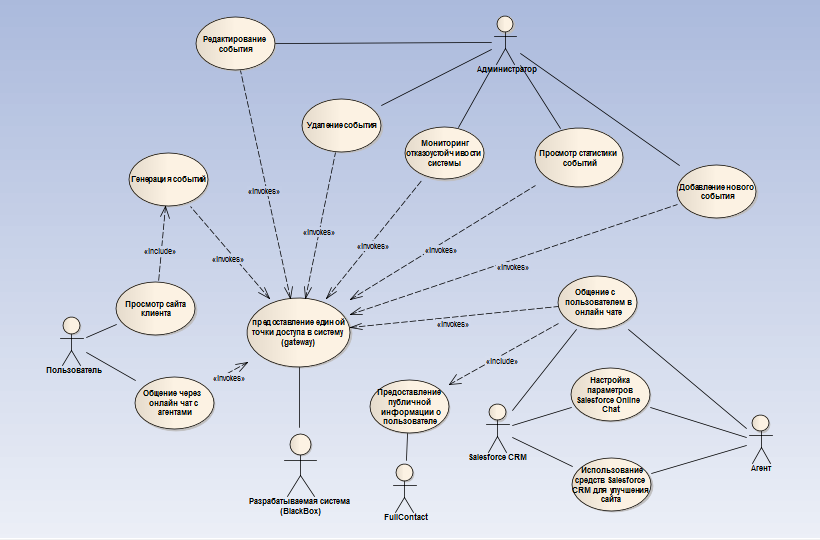
\includegraphics[scale=0.6]{uc-actors.png}  
  \caption{Функциональная модель}
	\label{fig:uc-actors}
\end{figure} 

Функциональная модель представлена на (рисунке~\ref{fig:uc-actors}).

На основании представленной диаграммы функциональной модели можно сделать вывод, что в системе будет существовать как минимум 6 актеров:
\begin{itemize}
\item пользователь;
\item агент;
\item администратор;
\item Salesforce CRM;
\item FullContact;
\item разрабатываемая система (BlackBox).
\end{itemize}
 
Рассмотрим каждого актера с его функциями более подробно.


Пользователь -- у пользователя в данной системе только две функции: он просматривает сайт (и тем самым генерирует события) и общается в онлайн чате с агентом.

Агент -- агент работает в Salesforce CRM. Он настраивает параметры для Salesforce Online Chat для отдельных страниц сайта, со своими особыми правилами появления чата, непосредственно общается с пользователем сайта, чтобы помочь последним и использует средства Salesforce CRM для улучшения сайта в результате диалога с пользователем.

Администратор -- настраивает систему отслеживания событий (добавляет/удаляет/редактирует события), следит и просматривает статистики происходящих событий для того чтобы понять как можно улучшить сайт. Также администратор наблюдает за отказоустойчивостью системы, чтобы в случае непредвиденных сбоев (потеря сети или интернета, выхода из строя серверов) быть готовым среагировать на возникшую проблему.

Salesforce CRM -- внешняя система, благодаря интеграции с которой, возникает возможность многофункционального онлайн чата с пользователем, а также возможность использования информации от него.

FullContact -- внешняя система, благодаря интеграции с которой, можно получить доступную публичную информацию о пользователе.

Разрабатываемая система (BlackBox) -- система, которая позволит всем перечисленным выше актерам выполнить свои функции. Она будет подробно рассмотрена в разделе ~\ref{sub:design:ps}  (рисунок~\ref{fig:uc-services}).


\subsection{Спецификация функциональных требований}
\label{sub:models:func_req}

Таким образом основной целью данного проекта является создание программного средства, позволяющего легко внедрять и использовать другие внешние сервисы и интегрировать их друг с другом.

В ходе разработки будут реализованы следующие возможности:
\begin{itemize}
\item интеграция с онлайн чатом CRM Salesforce;
\item создание системы отслеживания событий (event tracking system);
\item возможность настраивать онлайн чат с агентами определенных типов в зависимости от страницы сайта, на которой он должен появляться;
\item возможность настраивать онлайн чат так, чтобы сначала пользователь говорил с агентом одного типа (например обслуживающим лицом), а потом его, по результату разговора, можно было перенаправить на агента другого типа (например продавца);
\item возможность отслеживать процесс перехода состояний онлайн чата с помощью системы отслеживания событий;
\item возможность в панели администратора настраивать модели событий (создания/редактирования/удаления), которые сможет обрабатывать система отслеживания событий; 
\item возможность отслеживать действия пользователя на сайте с помощью системы отслеживания событий;
\item возможность в панели администратора просмотра (online/offline) статистики происходящих событий;
\item создание сервиса для нахождения публичной информации о пользователе с помощью интеграции с FullContact;
\end{itemize}

\subsection{Спецификация нефункциональных требованиями}
\label{sub:models:func_non_req}

Программное средство должно обладать следующими нефункциональными требованиями:
\begin{itemize}
\item работать в любом современном браузере(Chrome 40+, IE9+, Safari 7.7+, Firefox 3.6+);
\item интегрироваться с помощью js сниппета;
\item быть легковесным  и иметь как можно меньше накладных расходов для систем клиентов (подгружаемые скрипты должны быть < 10kb);
\item иметь интуитивно понятный интерфейс для просмотра статистик, чтобы новый пользователь мог его освоить за 2-3 дня;
\item иметь возможность легко включаться, выключаться и удаляться из систем клиентов;
\item иметь задержку не более 200ms при обращении к сервисам;
\item иметь возможность горизонтально масштабировать отдельные компоненты системы;
\item иметь возможность просмотра состояний отдельных компонентов системы;
\item иметь возможность работать с большим объемом поступающих входных данных (гигабайтами в день).
\end{itemize}
